\documentclass[journal]{IEEEtran}
\usepackage[a5paper, margin=10mm, onecolumn]{geometry}
%\usepackage{lmodern} % Ensure lmodern is loaded for pdflatex
\usepackage{tfrupee} % Include tfrupee package

\setlength{\headheight}{1cm} % Set the height of the header box
\setlength{\headsep}{0mm}     % Set the distance between the header box and the top of the text

\usepackage{gvv-book}
\usepackage{gvv}
\usepackage{cite}
\usepackage{amsmath,amssymb,amsfonts,amsthm}
\usepackage{algorithmic}
\usepackage{graphicx}
\usepackage{textcomp}
\usepackage{xcolor}
\usepackage{txfonts}
\usepackage{listings}
\usepackage{enumitem}
\usepackage{mathtools}
\usepackage{gensymb}
\usepackage{comment}
\usepackage[breaklinks=true]{hyperref}
\usepackage{tkz-euclide} 
\usepackage{listings}
% \usepackage{gvv}                                        
\def\inputGnumericTable{}                                 
\usepackage[latin1]{inputenc}                                
\usepackage{color}                                            
\usepackage{array}                                            
\usepackage{longtable}                                       
\usepackage{calc}                                             
\usepackage{multirow}                                         
\usepackage{hhline}                                           
\usepackage{ifthen}                                           
\usepackage{lscape}
\begin{document}

\bibliographystyle{IEEEtran}
\vspace{3cm}

\title{12.9.1.10}
\author{EE24BTECH11009 - Mokshith Kumar}
\maketitle

\textbf{Question:}\\
Solving the second-order differential equation:
\begin{align}
y'' + 2y' + \sin{y} = 0
\end{align}

\textbf{Solution:}\\
We aim to solve the second-order differential equation \( y'' + 2y' + \sin(y) = 0 \) using the Trapezoidal Method. To do so, we first convert the second-order differential equation into a system of first-order differential equations.

Let:
\begin{align}
v = y' \quad \text{(first derivative of \( y \))}\\
\end{align}
Then:
\begin{align}
v' = y'' \quad \text{(second derivative of \( y \))}
\end{align}
Substitute \( y' = v \) into the original differential equation:
\begin{align}
v' + 2v + \sin(y) = 0
\end{align}
This simplifies to the following system of first-order equations:
\begin{align}
\frac{dy}{dx} &= v\\
\frac{dv}{dx} &= -2v - \sin(y)
\end{align}
The Trapezoidal Method is an implicit method for numerically solving differential equations. It is based on averaging the slope at the current and next time steps, which results in the following update formulas:\\
For \( y \), we use the trapezoidal approximation:
\begin{equation}
    y_{n+1} = y_n + \frac{h}{2} \left( v_n + v_{n+1} \right)
\end{equation}
where \( h \) is the step size, and \( v_n \) and \( v_{n+1} \) are the values of \( v \) at the current and next time steps, respectively.\\
For \( v \), we also use a trapezoidal approximation for the derivative of \( v \):
\begin{equation}
    v_{n+1} = v_n + \frac{h}{2} \left( (-2v_n - \sin(y_n)) + (-2v_{n+1} - \sin(y_{n+1})) \right)
\end{equation}
This equation implicitly defines \( v_{n+1} \), so we need to solve for \( v_{n+1} \) at each step.\\

These are the difference equations used for solving the system of equations numerically. To solve for \( v_{n+1} \), we need to rearrange the second equation into an explicit form for \( v_{n+1} \).\\

Rearranging the second equation:
\begin{align}
    v_{n+1} - \frac{h}{2} \cdot (-2v_{n+1} - \sin(y_{n+1})) &= v_n + \frac{h}{2} \cdot (-2v_n - \sin(y_n)) \\
    v_{n+1} \left( 1 + h \right) &= v_n + \frac{h}{2} \left( -2v_n - \sin(y_n) - \sin(y_{n+1}) \right) \\
    v_{n+1} &= \frac{v_n + \frac{h}{2} \left( -2v_n - \sin(y_n) - \sin(y_{n+1}) \right)}{1 + h}
\end{align}

Now, we have a difference equation that we can solve numerically for \( v_{n+1} \).\\
\textbf{Verifying with Euler method :}\\
An exact theoretical solution using known methods to solve differential equations was not found. Therefore, we will use the numerical method(Euler method) to compare the solution, Which is my previous solution for this question.\\
We consider the initial conditions as follows:
$$
    \\x_0 = 0.0,\\y_0 = 1.0,\\v_0 = 1.0,\\ h = 0.01\\
$$
These initial conditions will help to start the numerical method.\\
The following plot is obtained from the above data.
\begin{figure}[h!]
   \centering
   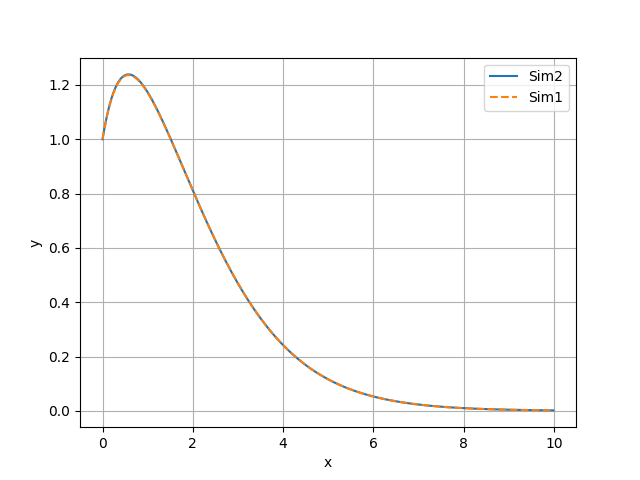
\includegraphics[width=\columnwidth]{figs/12.9.1.10.png}
   \caption{Plot of the computational solution of $y'' + 2y' + \sin(y) = 0$.}
   \label{}
\end{figure}
\end{document}
